% -----------------------------------------------
% Template for ISMIR 2010
% (based on earlier ISMIR templates)
% -----------------------------------------------

\documentclass{article}
\usepackage{ismir2010,amsmath,cite}
\usepackage{graphicx}
\usepackage{url}
\usepackage{algorithm,algorithmic}


% Title.
% ------
\title{Large-scale harmonic patterns clustering}

% Single address
% To use with only one author or several with the same address
% ---------------
%\oneauthor
% {Names should be omitted for double-blind reviewing}
% {Affiliations should be omitted for double-blind reviewing}

% Two addresses
% --------------
%\twoauthors
%  {First author} {School \\ Department}
%  {Second author} {Company \\ Address}

% Three addresses
% --------------
\threeauthors
  {First author} {Affiliation1 \\ {\tt author1@ismir.edu}}
  {Second author} {\bf Retain these fake authors in\\\bf submission to preserve the formatting}
  {Third author} {Affiliation3 \\ {\tt author3@ismir.edu}}
% what order do we use? Thierry, Ron, Dan? is Juan on?


\begin{document}
%
\maketitle
%
\begin{abstract}
We present a method for discovering typical patterns in music.
Similar to the \textit{shingle} idea, but done on a larger scale through
Echo Nest API, we cluster harmonic patterns from 43K songs. Patterns are
made of ordered chroma features, and not of summarization like gaussian
mixtures coefficients or NMF weights. We explain
how to operate on such large datasets, we analyze the obained clusters,
and we discuss there use for retrieval and encoding. All code is made
available.\\
TAKE-HOME MESSAGE: \textit{Shingles} idea can go large-scale?
\end{abstract}
%
\section{Introduction}\label{sec:introduction}

Working with large amount of audio data is a goal and a challenge at the
same time. One of the most common task is to find the nearest neighbor,
based on some distance, to a given segment of music. This can be viewed
as \textit{retrieval} as you are looking for some specific target
based on some query. $k$-nearest neighbors ($k$nn) algorithms have been
designed for that purpose, and recent improvements let them scale to
considerable data set sizes \cite{Datar2004}. The \textit{Shingles}
were introduced in that framework \cite{Casey2006}. A \textit{Shingle}
is a pattern of stacked chroma features. Similarity between
\textit{Shingles} coresponds to comparing harmonic patterns. For this
reason, they were used for cover or remix recognition \cite{Casey2007}.

That being said, nearest neighbor search is only one aspect of the
analysis of large-scale music data sets. Finding $k$ neighbors for a
particular query does not tell you much about the music space.
Clustering is a larger and more flexible framework where the goal is
to divide the space in meaningful blocks. The starting point is not
a query, but all the data itself. In this work, we bring the
\textit{Shingle} idea into that framework in order to discover
meaningful and typical music harmonic patterns. The underlying assumption
is that the music space is articulated around a certain number of
frequent patterns.

Note that clustering and neighbor search are not unrelated.
In practise, we would hope that close neighbors live in one or two
close clusters, thus clustering can be a preprocess step. Also,
knowing all $k$ neighbors of each sample let you do graph clustering,
a subset of the clustering algorithms.

A major component of this work is scalability. We experiment with a training
set of $43$ thousands song, but everything scales linear in time
relative to the number of samples. We could imagine, as an extension
of this work, an algorithm ``listening'' to all music it can find online.
Time would be an issue, but not memory.



\iffalse % ignored section
The original goal of the \textit{Shingles} was retrieval, i.e. find very
similar song segments based on their harmonic pattern. Part of the
challenge was to handle tons of overlapping song segments represented
by a rather long feature vector (a serie of chroma features).
The LSH algorithm proved a great solution for performing a $k$-nearest
neighbors ($k$nn) search in such a space. However, the paradigm of $k$nn has
an intrinsec scaling limit.

Finding a closest match is a tangible goal within a personal collection
of a few thousands songs. It can be used to discover cover songs or
find the seamless transitions in a playlist. However, the closest match
in millions and millions of music excerpts do not help us organize such
an amount of media. Some tasks are still important, for instance cover
recognition, and improvements in $k$nn methods are always welcome.
But it does not the describe the music space, nor does it necessarily
make good recommendations. We do not want to look for one neighbor, but
rather a cloud of potential close patterns. A similar argument in the 
recommendation domain is that precision becomes more important than recall 
passed a certain scale of data for many practical uses.

We propose to move the \textit{Shingle} idea into the larger clustering 
paradigm.
\fi % end of ignored section

The goal is to find typical patterns that can be seen as cluster centroids.
Those typical patterns help us understand a music collection from an
harmonic point of view. Segments of songs can be described in regard to their
proximity to the different centroids, thus creating some notion of distance
among the song segments. These cluster of similar patterns can have many usages:
\begin{enumerate}
\item describing the music space
\item finding potential similar songs and/or covers
\item eliminating quickly very wrong matches in a query system
\end{enumerate}

Our contribution is... large-scale clustering method, 


We present a practical way to do such large-scale clustering using vector
quantization. We present clustering results of an online algorithm on a data 
set of $43$K songs, but the method applies to any data size. We show how to
select different parameters such as the size of the \textit{Shingles} 
using an encoding scheme on a test set of $4$K songs. Finally, we illustrate
the method with some specific examples.


\subsection{Definitions}
A pattern, or a patch, is a \textit{Shingle} taken from an actual song.
A code is similar to a pattern, but is the result of the clustering
algorithm and most likely does not come from an actual song.
Distortion is our measure of distance between a pattern and a code.


\section{Previous Work}\label{sec:prevwork}
The idea is closely related to the \textit{Shingles} described by
Slaney and Casey \cite{Casey2006,Casey2007,Casey2008}. 

LSH: \cite{Datar2004}, LSH implementation: \cite{E2LSH}.
The E$^2$LSH packages can efficiently handle about $50$K or $100$K
vectors of size $200$. Even with a better implementation, the LSH
model still has some scaling problem. A large portion of the data
must be known to decide how many projections to use, and what guarantee
of finding the nearest neighbor it can provides. Also, we could fix the
number of projections and consider as clusters all the elements that
fall into the same bin. However, this does not give us a centroid, a
typical pattern representing that cluster.

Barrington et al. recently studied music texture using a set of ordered
MFCC vectors \cite{Barrington2009a}. This could be seen as complementary
to our work. Chromas capture the harmonic information and some of the
rythm while the MFCC are great timbral features.

Nearest neighbor and clustering methods are common in music similarity 
research, for instance \cite{Cano2004,Holzapfel2009}. The difference here 
are the actual patterns that we cluster.

Other large-scale work use summarization of the features. We mention 
gaussian mixtures \cite{Mandel2005}, aggregate features \cite{Bergstra2006a}
and linear dynamical systems \cite{Barrington2009a}. The chroma representation
is close from an harmonic point of view to the actual music, in particular
we can ``listen'' to the patches (see Section \ref{sec:experiments}).
This is an advantage for analyzing a large data set, and in accordance with our goal
we restrain ourselves from using generative models to compress our features.


\section{Data}\label{sec:data}
In this section we present our use of the Echo Nest features and the
datasets we use for training and testing our model.


\subsection{Echo Nest features}
We use the Echo Nest analyze API \cite{EchoNest} throughout this work.
The API gives us a chroma vector (length $12$) for every music event, 
or ``segment'', for any song we upload to their platform. 
We also get an estimate of where the beats and the bars are. 
We transform the chroma vectors per segment into per beat vector using a 
simple average. We can then stack beat vectors for a number of bars (usually 1 or 2). 
We get a fixed-size patch by resampling the number of chroma vectors. Typically,
there are $4$ beats per bar. Thus an appropriate patch size for one bar
is $12$x$4$ or $12$x$8$.

Note that we do not claim that any of these informations (segments, beats, bars)
are perfectly accurate (e.g. in \cite{Barrington2009a} authors improve on the
song segmentation features). Practise showed us that they are reasonable, 
and the size of the data set should make up for the imperfections or noise.
We also believe that patches sizes based on a number of beats or bars are more
meaningful than an arbitrary time length. More on this in the experiments
(Section \ref{sec:experiments}).


\begin{figure}[htb]
\begin{center}
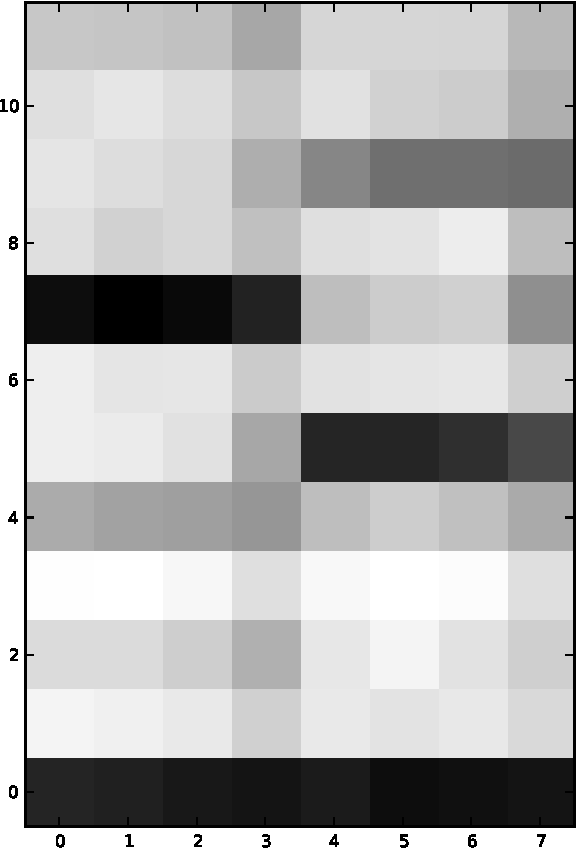
\includegraphics[width=.8\columnwidth]{code}
\end{center}
\caption{{A typical code from a code book of size $200$. Patterns represented
$2$ bars and the pattern length was set to $16$.}}
\label{fig:code}
\end{figure}

\subsection{Cowbell Dataset}
We have $43,300$ songs, giving  $3,720,091$ non zero bars, a bar usually 
contains $4$ beats.


\subsection{uspop2002}
We had acces to a low quality (32kbps) version of the songs in the uspop 2002 
data set \cite{uspop2002}.
This well-known data show a great diversity of pop songs, but is not particular
otherwise. We also tried to use Tzanetakis dataset \cite{Tzanetakis2002a}, but 
the $30$ seconds segments seemed hard to analyze by the Echo Nest API, most did
not contain any bar.

uspop2002 serves as testing set to measure how well a code book learned on
the Cowbell data set can represent new songs. We get Echo Nest features
for $8651$ songs from that dataset.

\section{Algorithm}\label{sec:algo}
In this section we present the creation of the harmonic patterns from
the Echo Nest data. Then, we explain the online vector quantization algorithm
used to learn a code book of those patterns.

\subsection{Pattern Creation}
Here we should explain key invariance, resizing, etc, and not in the
experiment section.


\subsection{Codebook Learning}
We use an online version of the vector quantization algorithm 
\cite{Gersho1991}. This can also be seen as an online Kmeans.
The idea is as follow: take a sample from your data, find the closest
code in the codebook, bring that code closer to the sample by some amount.
The details are explained as Algorithm \ref{algo:vq}. note that this
algorithm, though not optimal, is $O(n)$ with $n$ number of songs seen.
Thus it scales linearly to any size of data set. The setting of the learning
rate might become trickier, but this is not fundamentally a problem.


We initialize the codebook by choosing $K$ random points from our dataset.


\begin{algorithm}
%\caption{Pseudocode of Vector Quantization}
\label{algo:vq}
\begin{algorithmic}
\STATE$l$ learning rate
\STATE$\{P_n\}$ set of patches
\STATE$\{C_k\}$ codebook of $K$ codes
%\STATE $m \leftarrow b$
\REQUIRE $0 < l \leq 1$
\FOR{$nIters$}
\FOR{$p \in \{P_n\}$}
\STATE$c \leftarrow min_{c \in C_k} dist(p,c)$
\STATE$c \leftarrow c + (p - c) * l$
\ENDFOR
\ENDFOR
\RETURN $\{C_k\}$
\caption{{Pseudocode of Online Vector Quantization. Note that we can replace
the number of iteration by a threshold on the distortion over some test set.}}
\end{algorithmic}
\end{algorithm}






\section{Experiments}\label{sec:experiments}

\subsection{Setting}\label{ssec:setting}
We take one or two bars, normalize the patches to size 4, 8, or 16.
We roll the patch to be invariant to the key (on the patch level, not on
the song level). We learn a codebook of size $K$ over the cowbell dataset 
using the VQ algorithm (Algorithm \ref{algo:vq}). A typical learning rate 
is $0.01$ for $20$ iterations over the whole dataset.

We use the codebook to encode our testing set (see Section \ref{sec:data}).
Each pattern is encoded with only one code. We can measure the average
distance between a pattern and its encoding. We can also measure the use
of the different codes.

\subsection{Pattern length}
See encoding experiments in Table \ref{tab:psize}.


% RESULTS
% 200codes, 2 bars, pSize=16, maxener, True, False, not scaled = 3.788
%                                             averaged on size = 
% 200codes, 2 bars, pSize=8, maxener, True, False, not scaled  = 3.135
%                                             averaged on size = 
% 200codes, 1 bars, pSize=4, maxener, True, False, not scaled  = 
%                                             averaged on size = 
% 200codes, 7 beats, pSize=7, maxener, True, False, not scaled = 2.771
%                                             averaged on size = 
% 200codes, 5 beats, pSize=5, maxener, True, False, not scaled = 2.397
%                                             averaged on size = 
% 200codes, 3 beats, pSize=3, maxener, True, False, not scaled = 
%                                             averaged on size = 
\begin{table}
\begin{center}
\begin{tabular}{|l|c|}
\hline
size & avg. dist \\ \hline \hline
1 bar (4) & \\
2 bars (8) & $$\\
2 bars (12) & $$\\
2 bars (16) & $$ \\ \hline
3 beats & \\
5 beats & $$\\
7 beats & $$\\ \hline
\end{tabular}
\end{center}
\caption{{Encoding score for different pattern sizes. We can select the
size of the patterns based on bars. In this case, we put the actual size
of the pattern in parentheses. If the pattern size is based on beats, the
size is the number of beats. Results are on the uspop dataset, not seen
during training.}}
\label{tab:psize}
\end{table}


\subsection{Data Size}
We are interesting to see how the amount of training data changes
the quality of our code.
We experiment with different data sizes for a fixed size of codebook and a 
fixed code length. The data points are chose randomly from the whole
data set.
Code length: 1 bar resized to size 4. Code book size: 100
We measure the distortion on our test set. We hope for some convergence.
See results in Figure \ref{fig:sizes}.

Our learning can overfit, which explain the bad scores of small datasets.
The larger the dataset, the smallest the chance to overfit.
We are looking for a size of dataset that guarantees us a good learning
process, while being unnecessary large.

$500$ samples per code in the code book seems a good data size, see
Figure \ref{fig:sizes} for size $50$K.

\begin{figure}[htb]
\begin{center}
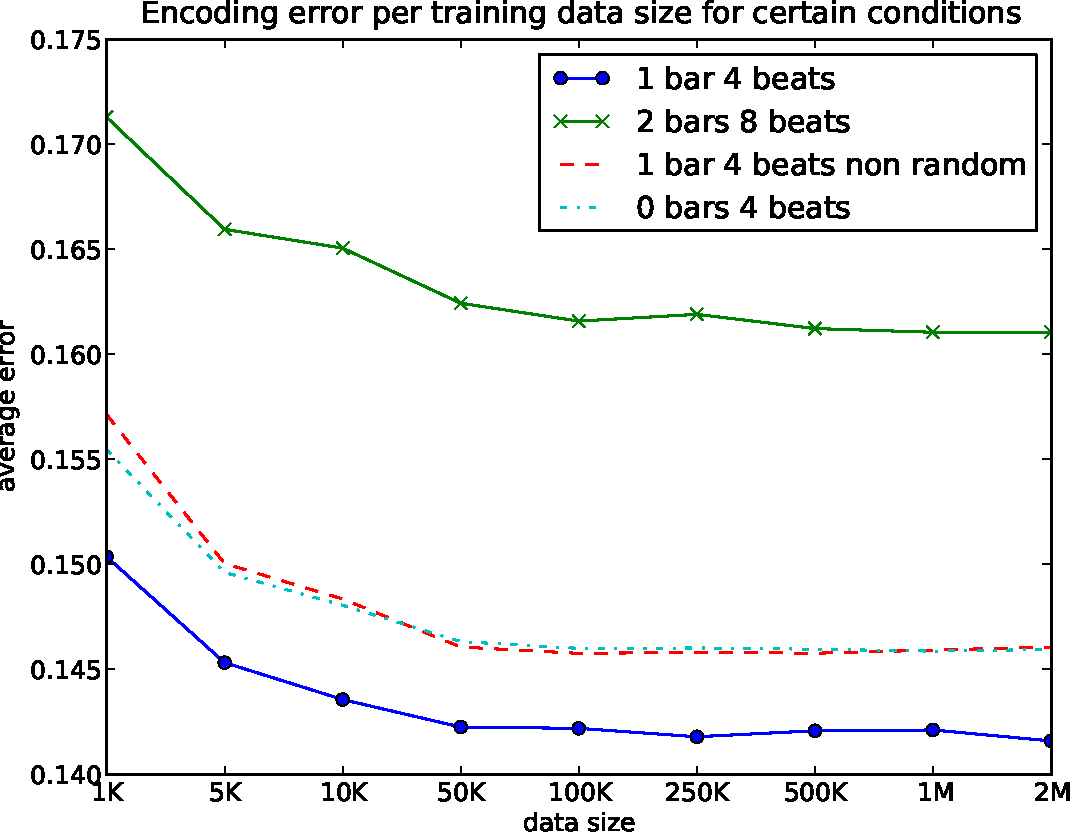
\includegraphics[width=.99\columnwidth]{data_sizes}
\end{center}
\caption{{Distortion for a code book of size $100$ encoding one bar
at a time, a bar being represented by $4$ chroma feature vector.
Therefore, a code or a pattern is of size $12$ x $4$ = $48$.
Distortion measure on the test data set. Data size tested range
from $10$ thousands to $2$ millions. Patterns were selected at
random from the dataset of approximately $3,7$ million patterns.}}
\label{fig:sizes}
\end{figure}

\iffalse
\begin{table}
\begin{center}
\begin{tabular}{|l|c|c|c|c|c|c|}
\hline
size & $5$K & $10$K & $50$K & $100$K & $500$K & $2$M  \\ \hline
distortion & $$ & $0.143$ & $0.142$ & $0.142$ & $0.142$ & $$\\ \hline
\end{tabular}
\end{center}
\caption{{Distortion for a code book of size $100$ encoding one bar
at a time, a bar being represented by $4$ chroma feature vector.
Therefore, a code or a pattern is of size $12$ x $4$ = $48$.
Distortion measure on the test data set. Data size tested range
from $10$ thousands to $2$ millions. Patterns were selected at
random from the dataset of approximately $3,7$ million patterns.}}
\label{tab:datasize}
\end{table}
\fi
% RESULTS:    
% 1bar s4     avg_distOLD    avg_dist
% 1K          0.150370
% 5K          0.145327
% 10K         0.143567
% 50K         0.142257
% 100K        0.142195
% 250K        0.141796
% 500K        0.142081
% 1M          0.142118
% 2M          0.141596
% 1bar s4 first X samples
% 1K          0.157142
% 5K          0.150045
% 10K         0.148357
% 50K         0.146069
% 100K        0.145765
% 250K        0.145819
% 500K        0.145772
% 1M          0.145924
% 2M          0.146065
% 0bar s4 (and test set same, we could do 1bar s4 in test set...)
% 1K          0.155474
% 5K          0.149619
% 10K         0.148056
% 50K         0.146328
% 100K        0.146004
% 250K        0.146024
% 500K        0.145962
% 1M          0.145873
% 2M          0.145955
% 2bar s8     
% 1K          0.171300
% 5K          0.165960
% 10K         0.165063
% 50K         0.162439
% 100K        0.161588
% 250K        0.161910
% 500K        0.161233
% 1M          0.161057
% 2M          0.161068


\subsection{Codebook Size}
Results in Table \ref{tab:cbsize}.

\begin{table}
\begin{center}
\begin{tabular}{|l|l|c|}
\hline
\# codes & \# samples & avg. dist \\ \hline \hline
1 & $500$ & $0.195939$ \\
10 & $5$K & $0.161812$ \\
50 & $25$K & $0.147472$ \\
100 & $50$K & $0.142194$ \\
200 & $100$K & $0.137548$ \\
500 & $250$K & $0.131211$ \\
1000 & $500$K & \\ \hline
\end{tabular}
\end{center}
\caption{{Code book size.}}
\label{tab:cbsize}
\end{table}
% RESULTS:      avg_distsOLD    avg_dist
% code 1        0.195939
% code 10       0.161812
% code 50       0.147472
% code 100      0.142194
% code 200      0.137548
% code 500      0.131211


\subsection{Codebook Size in Function of Pattern Length}
If the signal was totally random, and we were using 2 code to encode
every beat, we would need.... 4 codes for 2 beats? and 16 codes for
4 beats? and 256 codes for 8 beats?

Think about it in binary: two code to encode (0) and (1), but for
(0,0),(0,1),(1,0),(1,1) we need four codes for the same accuracy.

Reasonable size: 2 - 4 - 16 - 256. If we improve distance, music
is not random!

Then... 3 beats, 5 beats, 7 beats don't encode as well!

Special: 4 beats versus 1 bar - 4 beats, show the problem of being
not in sync with bars.

See code book size experiments in Table \ref{tab:cbsize}.

\begin{table}
\begin{center}
\begin{tabular}{|l|c|c|}
\hline
\# codes & \# bars & avg. dist \\ \hline \hline
2 & $1$ & $0.180750$ \\
4 & $2$ & $0.183631$ \\
16 & $4$ & $0.184078$ \\
256 & $8$ & $0.183464$ \\ \hline
2 & $2$ beats & $0.166840$ \\
4 & $1$ & $0.171495$ \\
16 & $2$ & $0.173767$ \\
256 & $4$ & $$ \\ \hline
\end{tabular}
\end{center}
\caption{{Code book size in function of the number of bars to encode.
All experiments done wtih $256 \times 500 = 128$K samples randomly chosen.}}
\label{tab:size_pattern}
\end{table}
% RESULTS:           avg_distsOLD   avg_dist
%2 codes 1 bar       0.180750       0.058435
%4 codes 2 bars      0.183631       0.054792
%16 codes 4 bars     0.184078       0
%256 codes 8 bars    0.183464       0
%---------------
%2 codes 2 beats     0.166840
%4 codes 1 bar       0.171495       
%16 codes 2 bars     0.173767
%256 codes 4 bars    0.174169


\subsection{Visualization}
We can use an algorithm like locally linear embedding \cite{Roweis2000} (LLE) 
or multidimensional scaling \cite{Kruskal1964} to visualize the data in
2 dimensions. We use the former\footnote{implementation: 
\url{http://www.astro.washington.edu/users/vanderplas/coding/LLE/}}, the
result can be seen in Figure \ref{fig:lle}.


\begin{figure}[htb]
\begin{center}
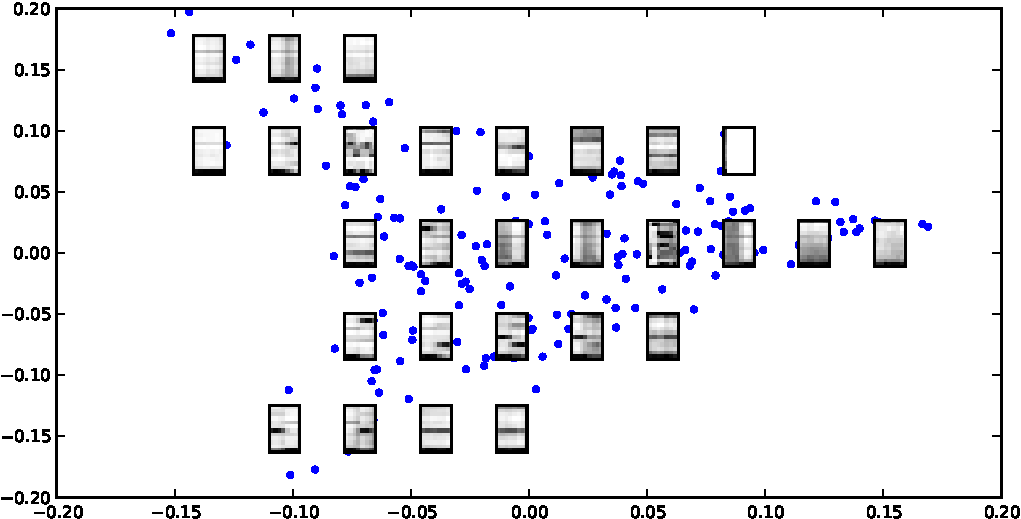
\includegraphics[width=.9\columnwidth]{codes_lle}
\end{center}
\caption{{LLE visualization of the code book.}}
\label{fig:lle}
\end{figure}

Another way is simply to present the codes in order of cluster size.
We encode the training or testing set as explained in Subsection 
\ref{ssec:setting} and we count how many patterns were closer to a particular
code than any other code. In Figure \ref{fig:firstcodes}, we show the $25$
most used codes out of a code book of size $200$.
Code from Figure \ref{fig:code} is the 37th most used code in that
code book. In Figure \ref{fig:closep}, we show a sample of patterns that
fall into its cluster.


\begin{figure}[htb]
\begin{center}
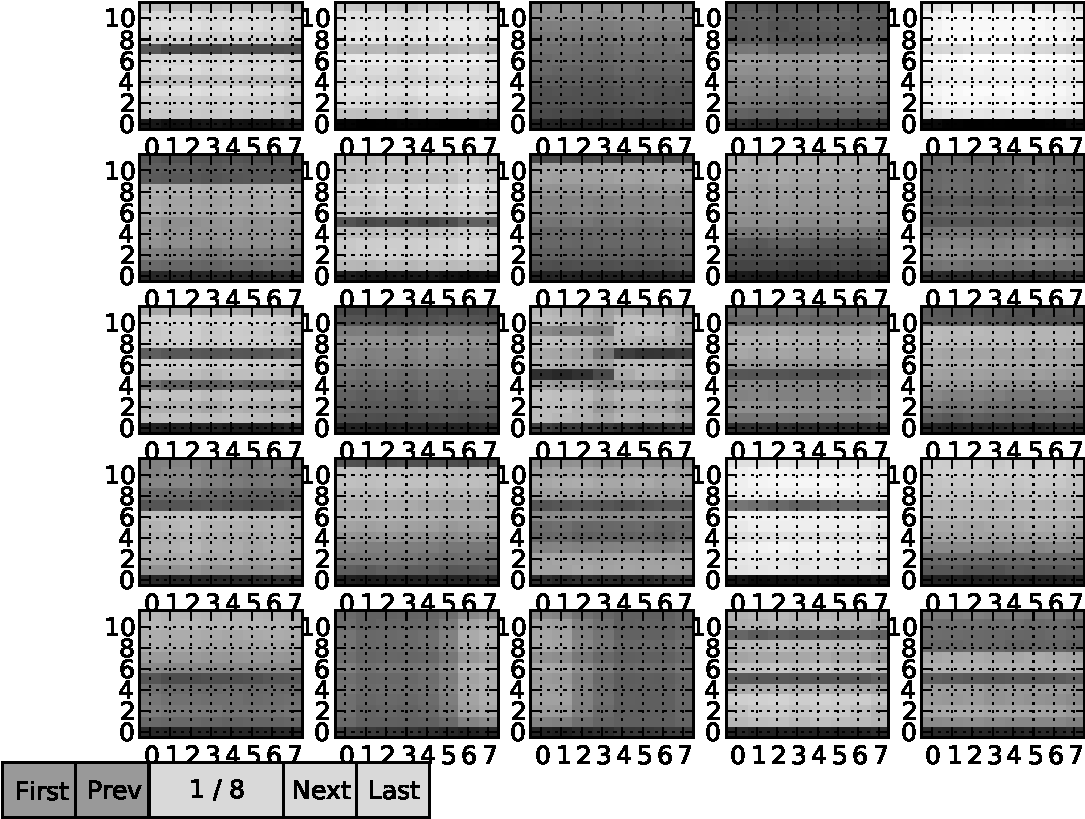
\includegraphics[width=.9\columnwidth]{codes1}
\end{center}
\caption{{$25$ most used codes on the training set.}}
\label{fig:firstcodes}
\end{figure}

The most common pattern is a sustained note, as we can see in Figure
\ref{fig:firstcodes}. Another common pattern is a sustained note
with an harmonic, as seen in the LLE visualization (Figure \ref{fig:lle}).

\begin{figure}[htb]
\begin{center}
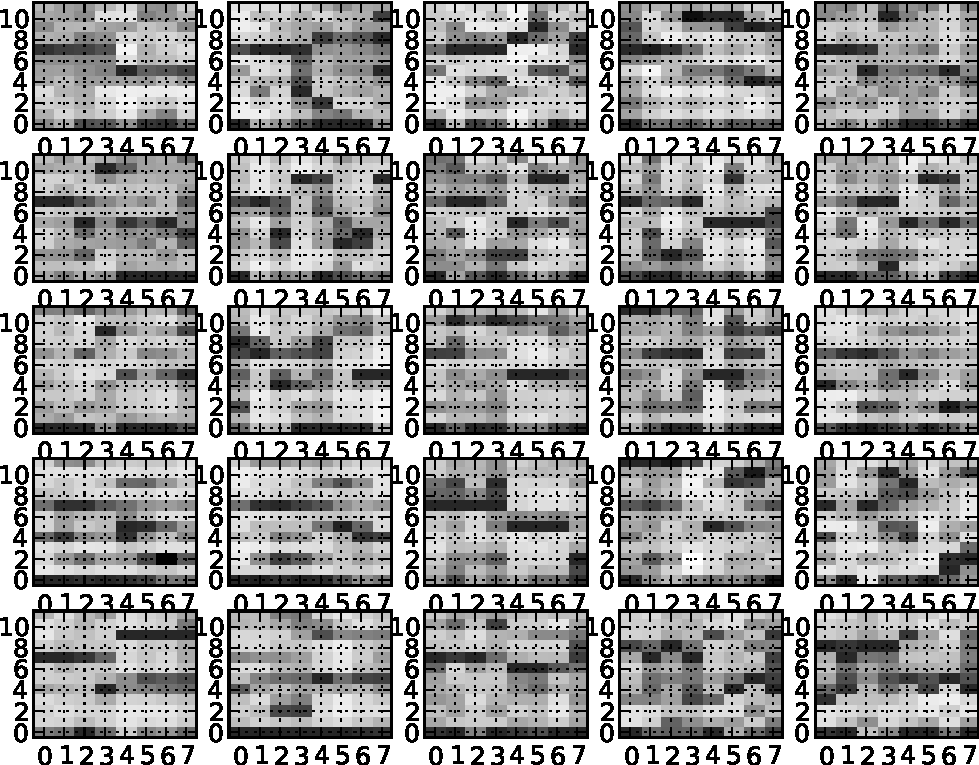
\includegraphics[width=.9\columnwidth]{close_patterns1}
\end{center}
\caption{{Sample of the close patterns to code in Figure \ref{fig:code}.}}
\label{fig:closep}
\end{figure}

\subsection{Specific Examples}


\section{Conclusion}
We are awesome. Here's how:
\begin{itemize}
\item large-scale
\item smarter shingles, based on beats and bars
\item clusters good for encoding
\item clusters good for something else?
\item free online API, code available\footnote{code not released yet to preserve 
submission's anonymity}
\item we have lab t-shirts
\end{itemize}

As for enhancements, we specifically did not compress our features using
gaussian mixtures or other generative model. That being said, these methods
could be use to develop better distance measures between \textit{Shingles}.
The use of the euclidean distance is arbitrary. Summarizing patches
with gaussians, and then comparing the distance between those gaussians,
could reduce the influence of the noise in the distance measure.



\small
%\section{Acknowledgements}
%Thierry is NSERC graduate fellow, or some title like that.


%\begin{thebibliography}{citations}
%\bibitem{Someone:04} 
%X. Someone and Y. Someone:
%{\it Title of the Book},
%Editorial Acme, Utrecht, 2004.
%\end{thebibliography}

\bibliography{tbm_bib}





\end{document}
